\section{\benchmark{}}
\label{sec:benchmark}
\benchmark{} is a benchmark featuring GitHub \textit{issues} from popular repositories that report bugs or request new features, and \textit{pull requests} that make changes to the repository to resolve these issues. 
The task is to generate a pull request that addresses a given issue and passes tests related to the issue.

\subsection{Benchmark Construction} 
\label{sec:benchmark:construction}
GitHub is a rich data source for software development, but repositories, issues, and pull requests can be noisy, ad-hoc, or poorly documented or maintained. 
To find high-quality task instances at scale, we use a $3$-stage pipeline as follows.

\begin{figure}[hb]
    \centering
    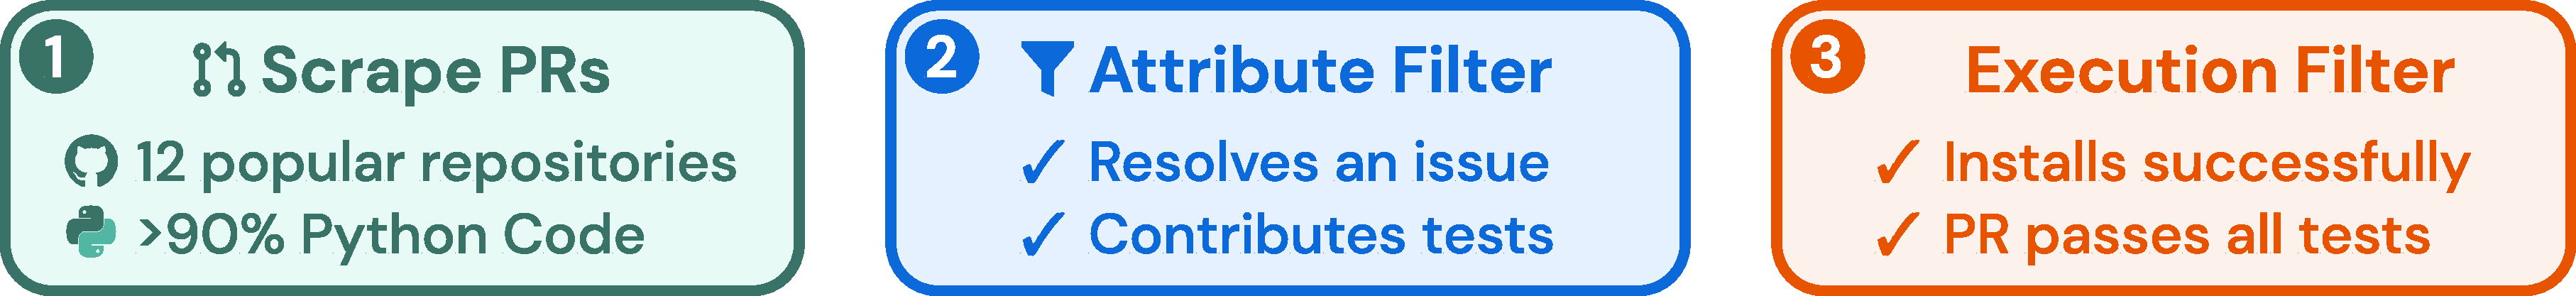
\includegraphics[width=0.85\linewidth]{figures/assets/collection-pipeline.pdf}
    \caption{
    \benchmark{} task instances are created from merged pull requests that resolve an issue, contributes tests, and install successfully.
    }
    \label{fig:collection-pipeline}
\end{figure}

\textbf{Stage I: Repo selection and data scraping}.
We start by collecting pull requests (PRs) from $12$ popular open-source Python repositories on GitHub, producing about $\sim\num{90000}$ PRs in total.
We focus on popular repositories as they tend be better maintained, have clear contributor guidelines, and have better test coverage.
Each PR has an associated codebase specified by it's base commit.

\textbf{Stage II: Attribute-based filtering}.
We create candidate tasks by selecting the \textit{merged} PRs that (1) resolve a GitHub issue and (2) make changes to the test files of the repository, which indicates that the user likely contributed tests to check whether the issue has been resolved.

\textbf{Stage III: Execution-based filtering}.
For each candidate task, we apply the PR's test content, and log the associated test results \textit{before} and \textit{after} the PR's other content is applied.
We filter out task instances without at least one test where its status changes from a \textit{fail} to \textit{pass} (henceforth referred to as \textit{fail-to-pass} test).
We also filter out instances that result in installation or runtime errors.

Through these stages of filtering, the original $\num{90000}$ PRs are filtered down to the $\num{2294}$ task instances which comprise \benchmark{}.
A final breakdown of these task instances across repositories is presented in Figure~\ref{fig:task-distribution}, and Table~\ref{table:dataset-stats} highlights the key features of \benchmark{} task instances. 
We highlight that the codebases are large with thousands of files, and the reference pull requests often make changes to multiple files at once.
Technical details about \benchmark{}'s construction pipeline are discussed in Appendix~\ref{appx:benchmark}.
Additional dataset statistics are in Appendix~\ref{appx:benchmark:repo-stats}.

\subsection{Task Formulation}
\label{sec:benchmark:task-formulation}

\textbf{Model input.}
A model is given an issue text description and a complete codebase.
The model is then tasked to make an edit to the codebase to resolve the issue.
In practice, we represent edits as patch files, which specify which lines in the codebase to modify in order to resolve the issue.

\textbf{Evaluation metrics.}
To evaluate a proposed solution, we apply the generated patch, using unix's \texttt{patch} program, to the codebase and then execute the unit and system tests associated with the task instance.
If the patch applies successfully and all of these tests pass we consider the proposed solution to have successfully resolved the issue.
The metric for our benchmark is the percentage of task instances that are resolved.
Additional technical details in Appendix~\ref{appx:benchmark:eval-procedure}.

\subsection{Features of \benchmark{}}
\label{sec:benchmark:features-of-benchmark}

Traditional benchmarks in NLP typically involve only short input and output sequences and consider somewhat ``contrived'' problems created specifically for the benchmark.
In contrast, \benchmark{}'s realistic construction setting imbues the dataset with unique properties, which we discuss below.

\textbf{Real-world software engineering tasks}.
Since each task instance in \benchmark{} consists of a large and complex codebase and a description of a relevant issue, solving \benchmark{} requires demonstrating sophisticated skills and knowledge possessed by experienced software engineers but are not commonly evaluated in traditional code generation benchmarks.

\textbf{Continually updatable}.
Our collection process can be easily applied to any Python repository on GitHub and requires minimal human intervention.
Therefore, we can extend \benchmark{} with a continual supply of new task instances and evaluate LMs on issues created after their training date, which ensures that the solution was not included in their training corpus.

\textbf{Diverse long inputs.}
Issue descriptions are typically long and detailed ($195$ words on average), and codebases regularly contain many thousands of files.
Solving \benchmark{} requires identifying the relatively small number of lines that need to be edited to solve an issue amongst a sea of context.

\textbf{Robust evaluation.}
For each task instance, there is at least one \textit{fail-to-pass} test which was used to test the reference solution, and $40\%$ of instances have at least two fail-to-pass tests.
These tests evaluate whether the model addressed the problem in the issue.
In addition, a median of $51$ additional tests run to check whether prior functionality is properly maintained.

\textbf{Cross-context code editing.}
Unlike prior settings that may constrain edit scope to an individual function or class~\citep[e.g.,][]{chen2021evaluating, cassano2022multiple} or provide \textit{cloze}-style fill-in blanks~\citep[e.g.,][]{lu2021codexglue,fried2023incoder}, \benchmark{} does not provide such explicit guidance.
Rather than merely having to produce a short code snippet, 
our benchmark challenges models to generate revisions in multiple locations of a large codebase.
\benchmark{}'s reference solutions average editing $1.7$ files, $3.0$ functions, and $32.8$ lines (added or removed).

\textbf{Wide scope for possible solutions.}
The task of repository-scale code editing can serve as a level playing field to compare approaches ranging from retrieval and long-context models to decision-making agents, which could reason and act in code.
\benchmark{} also allows creative freedom, as models can generate novel solutions that may deviate from the reference PR.

\begin{table}[t]
\begin{minipage}{.49\linewidth}
    \begin{minipage}{\textwidth}
        \centering
        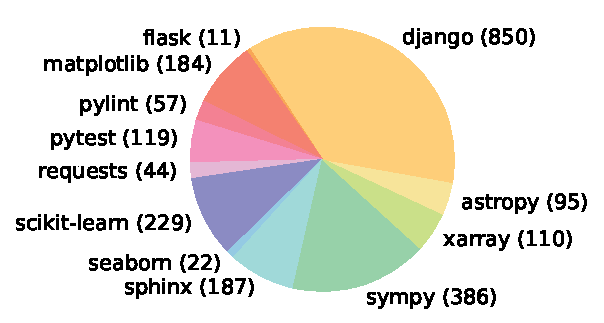
\includegraphics[width=\textwidth]{figures/assets/task-distribution.pdf}
        \captionof{figure}{
        Distribution of \benchmark{} tasks (in parenthesis) across 12 open source GitHub repositories that each contains the source code for a popular, widely downloaded PyPI package.
        }
        \label{fig:task-distribution}
    \end{minipage}
\end{minipage}
\hfill
\begin{minipage}{.48\linewidth}
    \begin{minipage}{\textwidth}
        \centering
        \caption{
        Average and maximum numbers characterizing different attributes of a \benchmark{} task instance.
        Statistics are micro-averages calculated without grouping by repository.
        }
        \resizebox{\textwidth}{!}{
        \small
        \begin{tabular}{llrr}
        \toprule
            & & Mean & Max \\
        \midrule
            Issue Text & Length (Words) & 195.1 & 4477 \\
            \midrule
            \multirow{2}{*}{Codebase} & \# Files (non-test) & 3,010 & 5,890 \\
                                      & \# Lines (non-test) & 438K  & 886K \\
            \midrule
            \multirow{3}{*}{Gold Patch} & \# Lines edited & 32.8 & 5888 \\
                                        & \# Files edited & 1.7 & 31 \\
                                        & \# Func. edited & 3 & 36 \\
            \midrule
            \multirow{2}{*}{Tests} & \# Fail to Pass & 9.1 & 1633 \\
                                   & \# Total & 120.8 & 9459 \\
        \bottomrule
        \end{tabular}
        }
        \label{table:dataset-stats}
    \end{minipage}
\end{minipage}
\vspace{-0.5em}
\end{table}


\subsection{\benchmark{} Lite}
Evaluating LMs on SWE-bench can be time-consuming and, depending on the model, require a costly amount of compute or API credits.
Given that initial performance returns as presented in Section~\ref{sec:results} are quite low, \benchmark{}'s difficulty makes it useful for gauging LM progress in the long term, but potentially intimidating for initial systems that attempt to make progress in the short term.
To encourage adoption of SWE-bench, we create a Lite subset of $300$ instances from SWE-bench that have been sampled to be more self-contained, with a focus on evaluating functional bug fixes.
The full filtering criteria and dataset information is included in 
SWE-bench Lite covers $11$ of the original $12$ repositories, with a similar diversity and distribution of task instances across repositories as the original.
Full details of the Lite split and filtering details are included in Appendix~\ref{appx:benchmark:lite}.